\documentclass{beamer}
\usepackage{fontspec} 
\usepackage{soul}
\usepackage{tikz}
\usepackage{pgfplots}
\newcommand{\barplot}[4]{%
  \begin{tikzpicture}
    \begin{axis}[
	xlabel={#1},  
	ylabel={#2}, 
	axis lines*=left, 
        width  = \textwidth,
	height = .3\textheight,
    	nodes near coords, 
	xtick=data,
	x tick label style={},  
	ymin=0,
	symbolic x coords={#3},
	]
	\addplot+[ybar,lsRichGreen!80!black,fill=lsRichGreen] plot coordinates {
	    #4
	}; 
    \end{axis} 
  \end{tikzpicture} 
}

\useoutertheme{lsp}

\usepackage{lsptitle}

\def\two@digits#1{\ifnum#1<10 0\fi\number#1}
\def\mytoday{\two@digits{\number\day}.\two@digits{\number\month}.\number\year}


\usepackage{xspace,multicol}
\newcommand{\latex}{\LaTeX\xspace}
\usepackage{tikz}


\newcounter{lastpagemainpart}
\footnotesep0pt
\renewcommand{\footnoterule}{}
\usefootnotetemplate{
  \noindent
  \insertfootnotemark\insertfootnotetext}

\let\beamerfn=\footnote
\renewcommand{\footnote}[1]{%
\let\oldfnsize=\footnotesize%
\let\footnotesize=\tiny%
\beamerfn<\thebeamerpauses->{#1}%
\let\footnotesize=\oldfnsize}


\date{13.6.2019}

\usepackage{eurosym}  
 
\renewcommand{\centerline}[1]{\hfill#1\hfill\hfill\mbox{}}


\title{Finanzierungsmodelle: \mbox{Praxisbeispiel Language Science Press}}
\institute{Language Science Press}
\author[LangSci]{Sebastian Nordhoff}



\begin{document}
\lspbeamertitle


\section{Introduction}
\frame{
\frametitle{Language Science Press}
\begin{itemize}
 \item aktiv seit 2014
 \begin{itemize}
   \item 2014--2016 FU Berlin 
   \item 2016--2018 HU Berlin
   \item 2019-- gemeinnützige UG
 \end{itemize}

 \item Monographien und Sammelbände in der Linguistik
 \item alle Bücher Open Access
 \item Stand heute 102 Bücher veröffentlicht
 \item Ziel: 30 Bücher/Jahr
 \item 25 Reihen; 1017 Supporter; 350 Community Proofreader
 \item Neben Linguisten und Programmierinnen auch eine Betriebswirtin in der Anfangsphase
\end{itemize}
}

\frame{
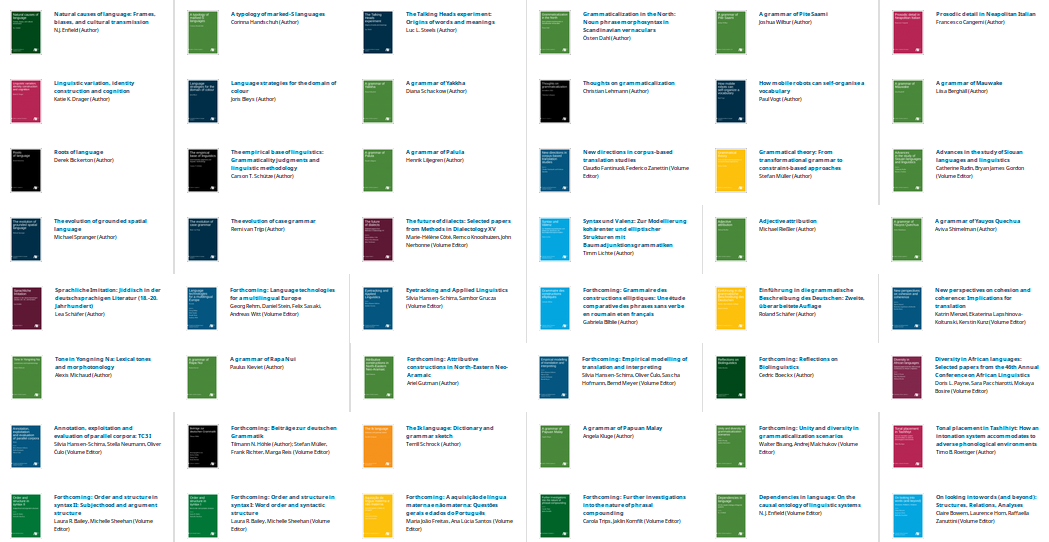
\includegraphics[width=\textwidth]{catalog.png}
}

\section{Geschäftsmodell}
\frame{
\frametitle{OpenAire non-BPC²}
 \textit{Full disclosure:  replicable strategies for book
publications supplemented with empirical data}\\

\includegraphics[width=.35\textwidth]{businessmodel.png}\hfill
\includegraphics[width=.35\textwidth]{cookbook.png}\hfill
~

\url{langsci-press.org/opendata}
}

\frame{
\frametitle{Frage \#1 beim Aufsetzen einer Publikationsplattform}
~
\pause
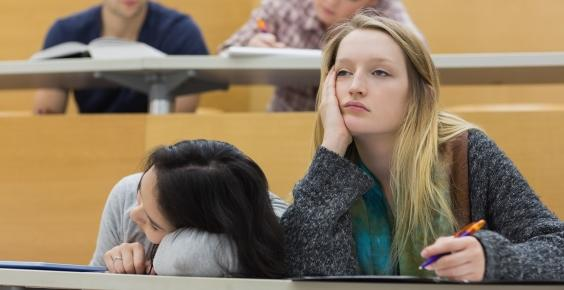
\includegraphics[width=\textwidth]{whocares.jpg}
\\[.7em] 

\pause {\hspace*{2cm} \LARGE Who cares?}
}

\frame{
\frametitle{Wen soll das denn\vphantom{fj}\\  interessieren?}
\begin{tabular}{ll}
 Leserinnen\vphantom{fj} & \\[1em]
 Autorinnen\vphantom{fj} & \\[1em]
 Institutionen\vphantom{fj} & \\[1em]
 Gesellschaft\vphantom{fj} & \\
\end{tabular}
}

\frame{
\frametitle{Konzipieren von\\ Finanzierungsströmen}
\begin{tabular}{l@{~${\Longleftarrow}$~}l}
 Leserinnen\vphantom{fj} & \fbox{\vphantom{fj}\st{Kauf/Abo}} \fbox{\vphantom{fj}Spenden} \fbox{\vphantom{fj}Mitgliedschaft}\\[1em]
 Autorinnen\vphantom{fj} & \fbox{\vphantom{fj}Autorengebühren} \fbox{\vphantom{fj}Mitgliedschaft}\\[1em]
 Institutionen\vphantom{fj} & \fbox{\vphantom{fj}institutionelle Mitgliedschaft}\\[1em]
 Gesellschaft\vphantom{fj} & \fbox{\vphantom{fj}geldgeberfinanzierte Plattform}\\
\end{tabular}
}


\frame{
\frametitle{Geschäftsmodell:\vphantom{fj}\newline 
Schätzwerte \& Projektionen} 
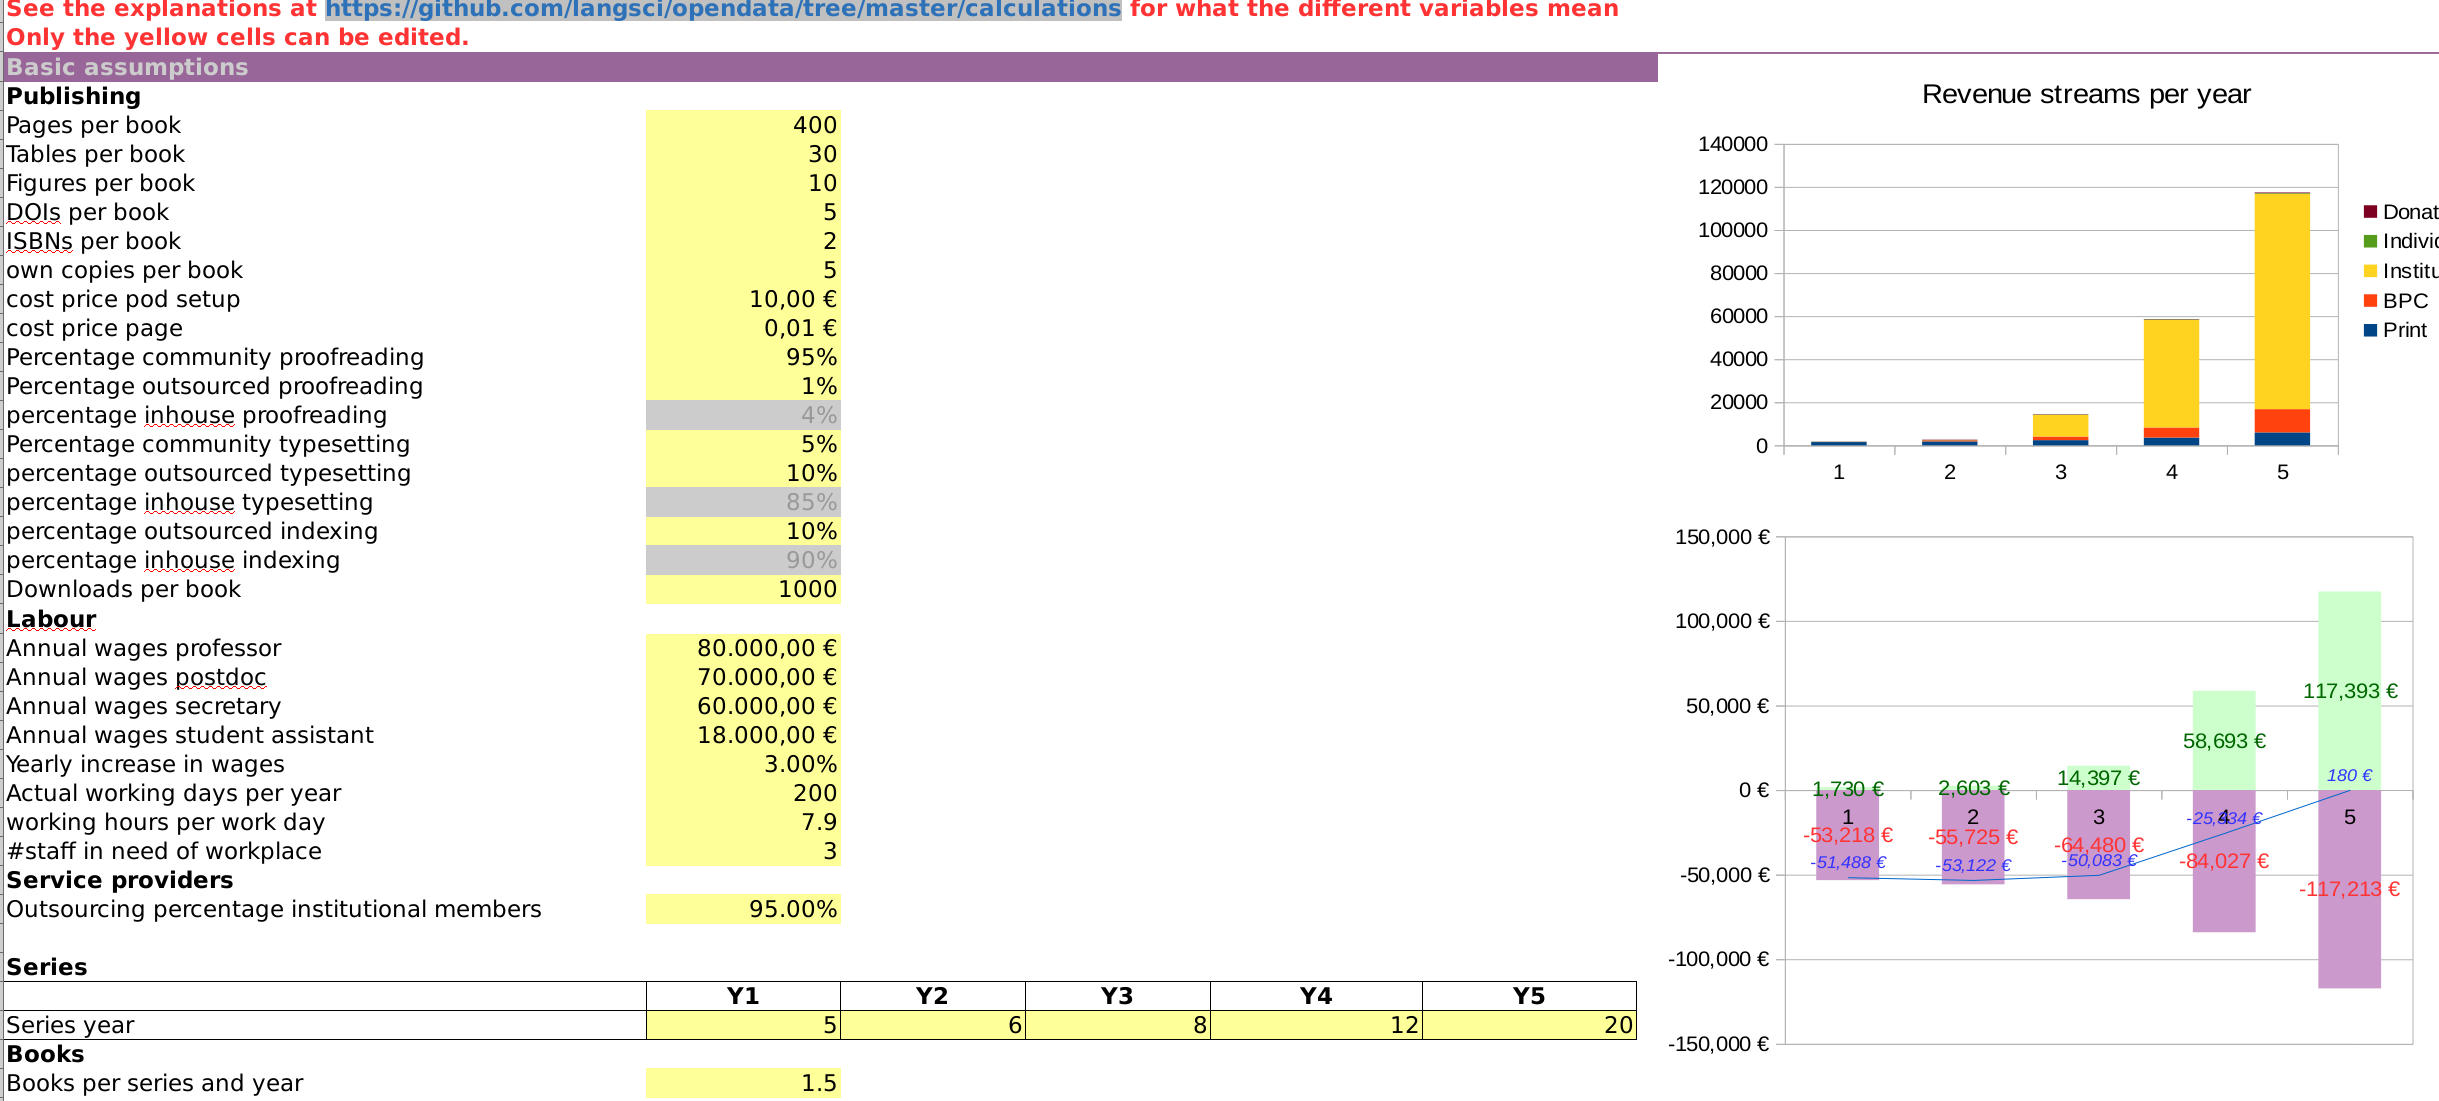
\includegraphics[width=\textwidth]{spreadsheet.png}
}


\frame{
\frametitle{Geschäftsmodell:\vphantom{fj}\newline Projektionen}
  \begin{tikzpicture}
    \begin{axis}[
      scaled y ticks = false,
	y tick label style={/pgf/number format/fixed,
	/pgf/number format/1000 sep = \thinspace % Optional if you want to replace comma as the 1000 separator 
	},    
	xlabel={Revenue stream},  
	ylabel={EUR}, 
	axis lines*=left, 
        width  = \textwidth,
	height = \textheight,
    	nodes near coords, 
	xtick=data,
	x tick label style={},  
	ymin=0,
	symbolic x coords={individual m, donations, print margin, BPCs, institutional m},
	]
	\addplot+[ybar,lsRichGreen!80!black,fill=lsRichGreen] plot coordinates {
	  (individual m, 13200)
	  (donations, 9600)
	  (print margin, 24000)
	  (BPCs, 25200)
	  (institutional m, 56000)
	}; 
    \end{axis} 
  \end{tikzpicture} 
}

\frame{
\frametitle{\mbox{Wunder der Bürokratie}}

\includegraphics[width=\textwidth]{bureaucracymagic.png}
}


\frame{
\frametitle{Geschäftsmodell: Evaluation}
  \begin{tikzpicture}
    \begin{axis}[
    scaled y ticks = false,
      y tick label style={/pgf/number format/fixed,
      /pgf/number format/1000 sep = \thinspace % Optional if you want to replace comma as the 1000 separator 
      },
	xlabel={Revenue stream},  
	ylabel={EUR}, 
	axis lines*=left, 
        width  = \textwidth,
	height = \textheight,
    	nodes near coords, 
	xtick=data,
	x tick label style={},  
	ymin=0,
	ybar,
	symbolic x coords={individual m, donations, print margin, BPCs, institutional m},
	]
	\addplot[ybar,lsRichGreen!80!black,fill=lsRichGreen] plot coordinates {
	  (individual m, 13200)
	  (donations, 9600)
	  (print margin, 24000)
	  (BPCs, 25200)
	  (institutional m, 56000)
	}; 
	\addplot[ybar,lsDarkBlue!60!black,fill=lsDarkBlue!60!black] plot coordinates {
	  (individual m, 120)
	  (donations, 3000)
	  (print margin, 6000)
	  (BPCs, 2500)
	  (institutional m, 0)
	}; 
    \end{axis} 
  \end{tikzpicture} 
}

\section{Evaluation}
\frame{
\frametitle{Geschäftsmodell: Evaluation}
  \begin{tikzpicture}
    \begin{axis}[
    scaled y ticks = false,
      y tick label style={/pgf/number format/fixed,
      /pgf/number format/1000 sep = \thinspace % Optional if you want to replace comma as the 1000 separator 
      },
	scaled y ticks=false
	tick label style={/pgf/number format/fixed}
	xlabel={Revenue stream},  
	ylabel={EUR}, 
	axis lines*=left, 
        width  = \textwidth,
	height = \textheight,
    	nodes near coords, 
	xtick=data,
	x tick label style={},  
	ymin=0,
	ybar,
	symbolic x coords={individual m, donations, print margin, BPCs, institutional m},
	]
	\addplot+[ybar,lsRichGreen!80!black,fill=lsRichGreen] plot coordinates {
	  (individual m, 13200)
	  (donations, 9600)
	  (print margin, 24000)
	  (BPCs, 25200)
	  (institutional m, 56000)
	}; 
	\addplot+[ybar,lsDarkBlue!60!black,fill=lsDarkBlue!60!black] plot coordinates {
	  (individual m, 120)
	  (donations, 3000)
	  (print margin, 6000)
	  (BPCs, 2500)
	  (institutional m, 85000)
	}; 
    \end{axis} 
  \end{tikzpicture} 
}



\frame{
\frametitle{Sharing is caring: GitHub} 
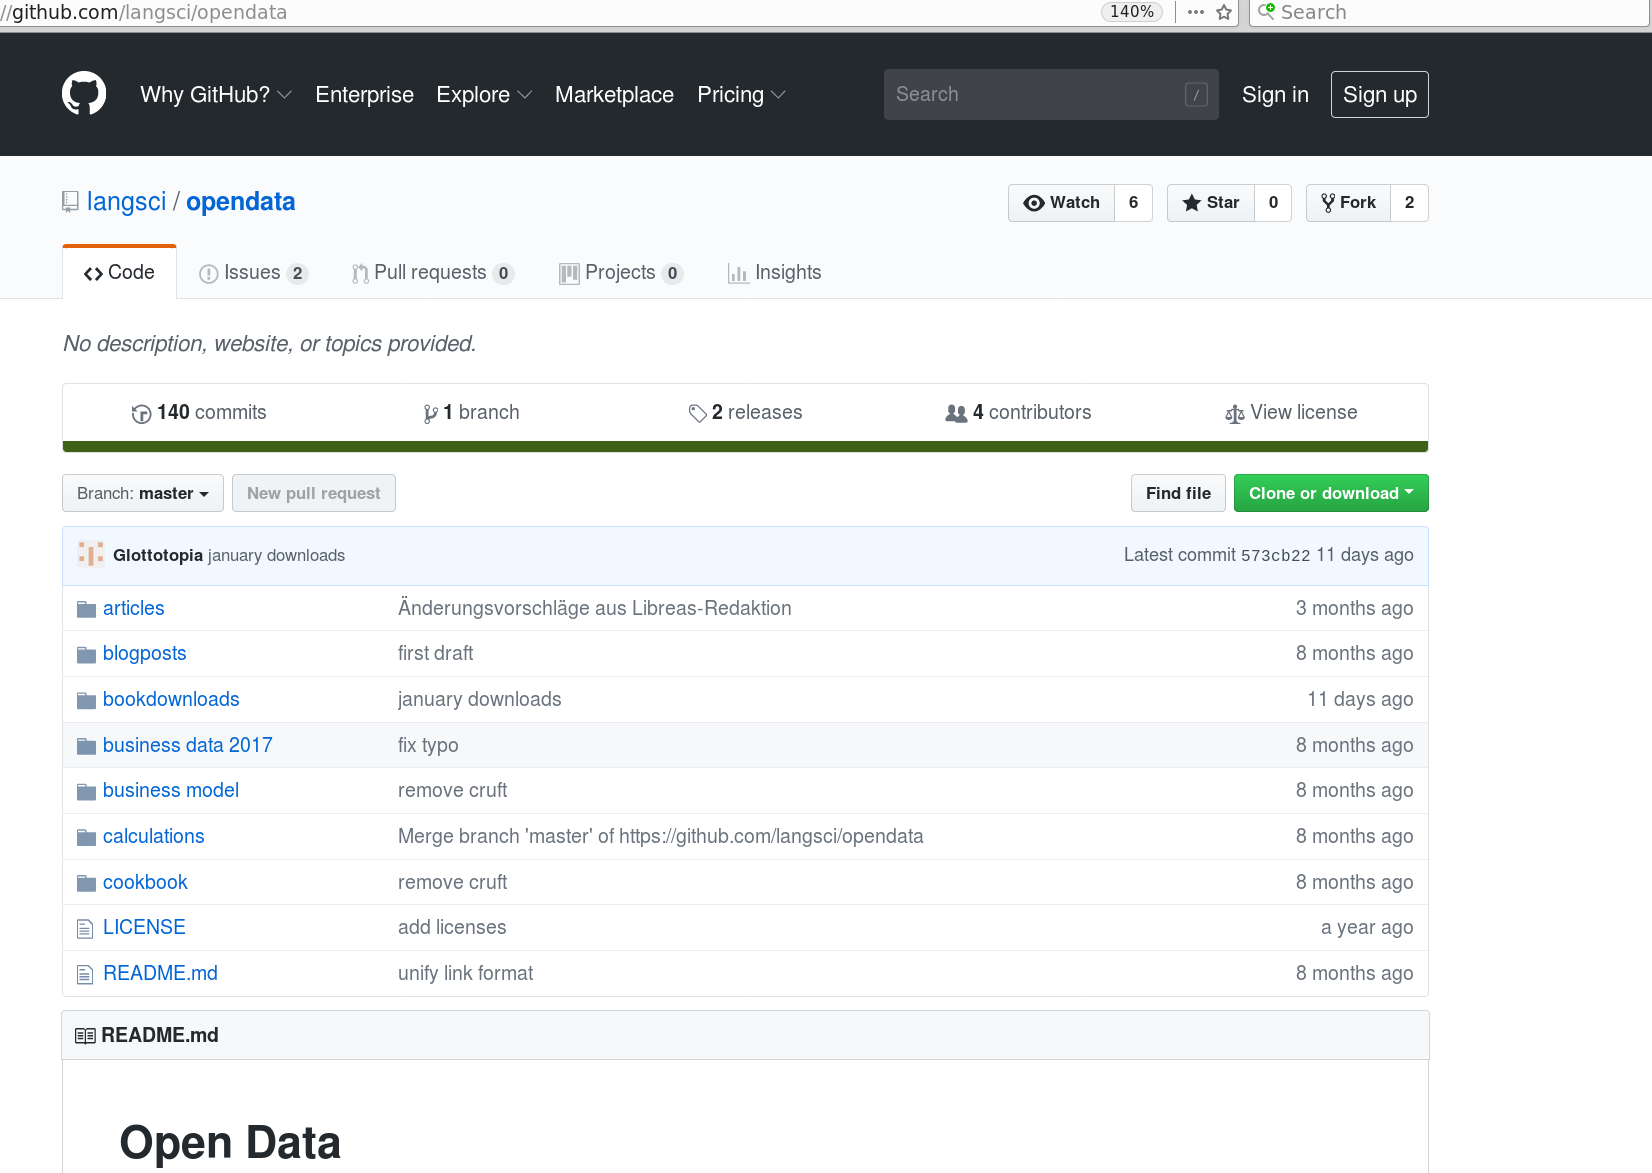
\includegraphics[width=\textwidth]{github.png}
}

\frame{
\frametitle{Sharing is caring:\newline Tabellenkalkulation} 
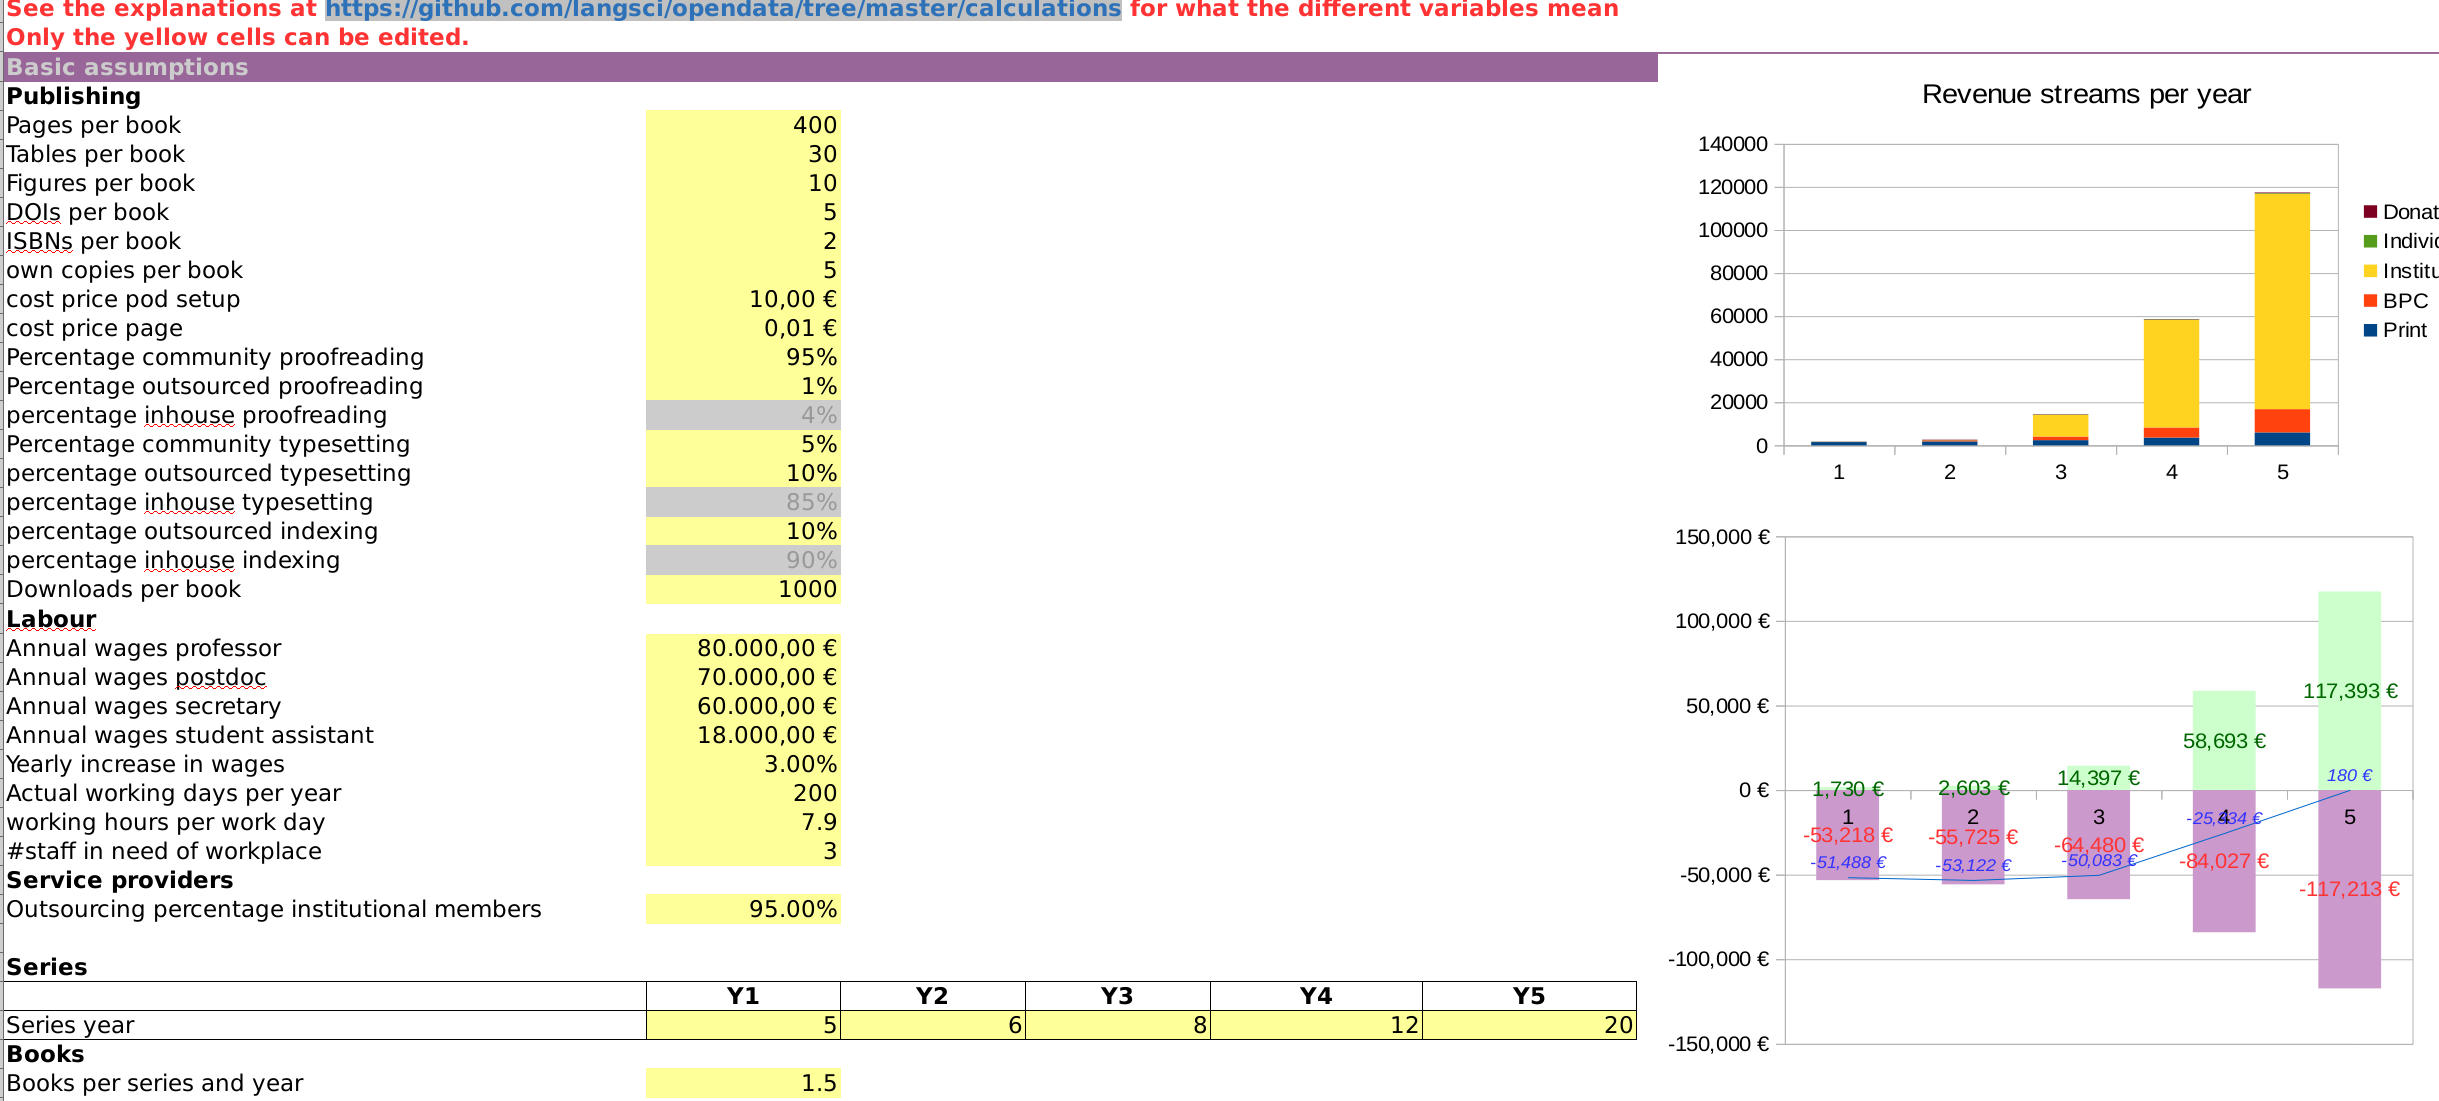
\includegraphics[width=\textwidth]{spreadsheet.png}
\url{https://github.com/langsci/opendata/blob/master/calculations/5y-setup.ods}
}



% \frame{
% \frametitle{But what if this does not work for me?}
% \begin{itemize}
%  \item work on alternatives
%  \item specify the alternatives 
%  \item evaluate the alternatives 
%  \item share the alternatives
%  \begin{itemize}
%   \item best practices, lessons learned
%  \end{itemize}
% \end{itemize}
% }

\frame{

\includegraphics[width=.4\textwidth]{businessmodel.png}\hfill
\includegraphics[width=.4\textwidth]{cookbook.png}\hfill
~
\url{langsci-press.org/opendata}
}

\frame{
\frametitle{Derzeitige Kosten}
%   \includegraphics[height=.2\textheight]{./path/to/graphicsfile}
  \begin{itemize}
    \item ca. 100\,000 EUR/Jahr
    \item mehr als 2/3 Personalkosten
    \item ca. 3\,500 EUR pro Buch bei Language Science Press 
    \item diverse Studien führen Kosten von 15\,000 bis 130\,000 EUR pro Buch an 
    \item allgemein sollten je nach Fachgebiet 5\,000--8\,000 EUR erreichbar sein
    \item Voraussetzung: ordentliche Kalkulation und Evaluation
  \end{itemize}
}

\frame{
\frametitle{Derzeitige Finanzierung}
%   \includegraphics[height=.2\textheight]{./path/to/graphicsfile}
  \begin{itemize}
    \item  Institutionelle Mitgliedschaften
    \begin{itemize}
      \item Knowledge Unlatched als Vermittler 
      \item 15\% Kommission
    \end{itemize}
    \item 105 Institutionen @ 1000 EUR/Jahr
    \item 2018--2020; 2021--2023; 2024--2026; ...
    \item Problem: Wachstum
    \begin{itemize}
      \item mehr Institutionen? 
      \item höhere Beträge? 
      \item gestaffelte Beträge? 
      \item doch noch andere Geldströme?
    \end{itemize}

  \end{itemize}
}

\frame{
\frametitle{Vielen Dank}
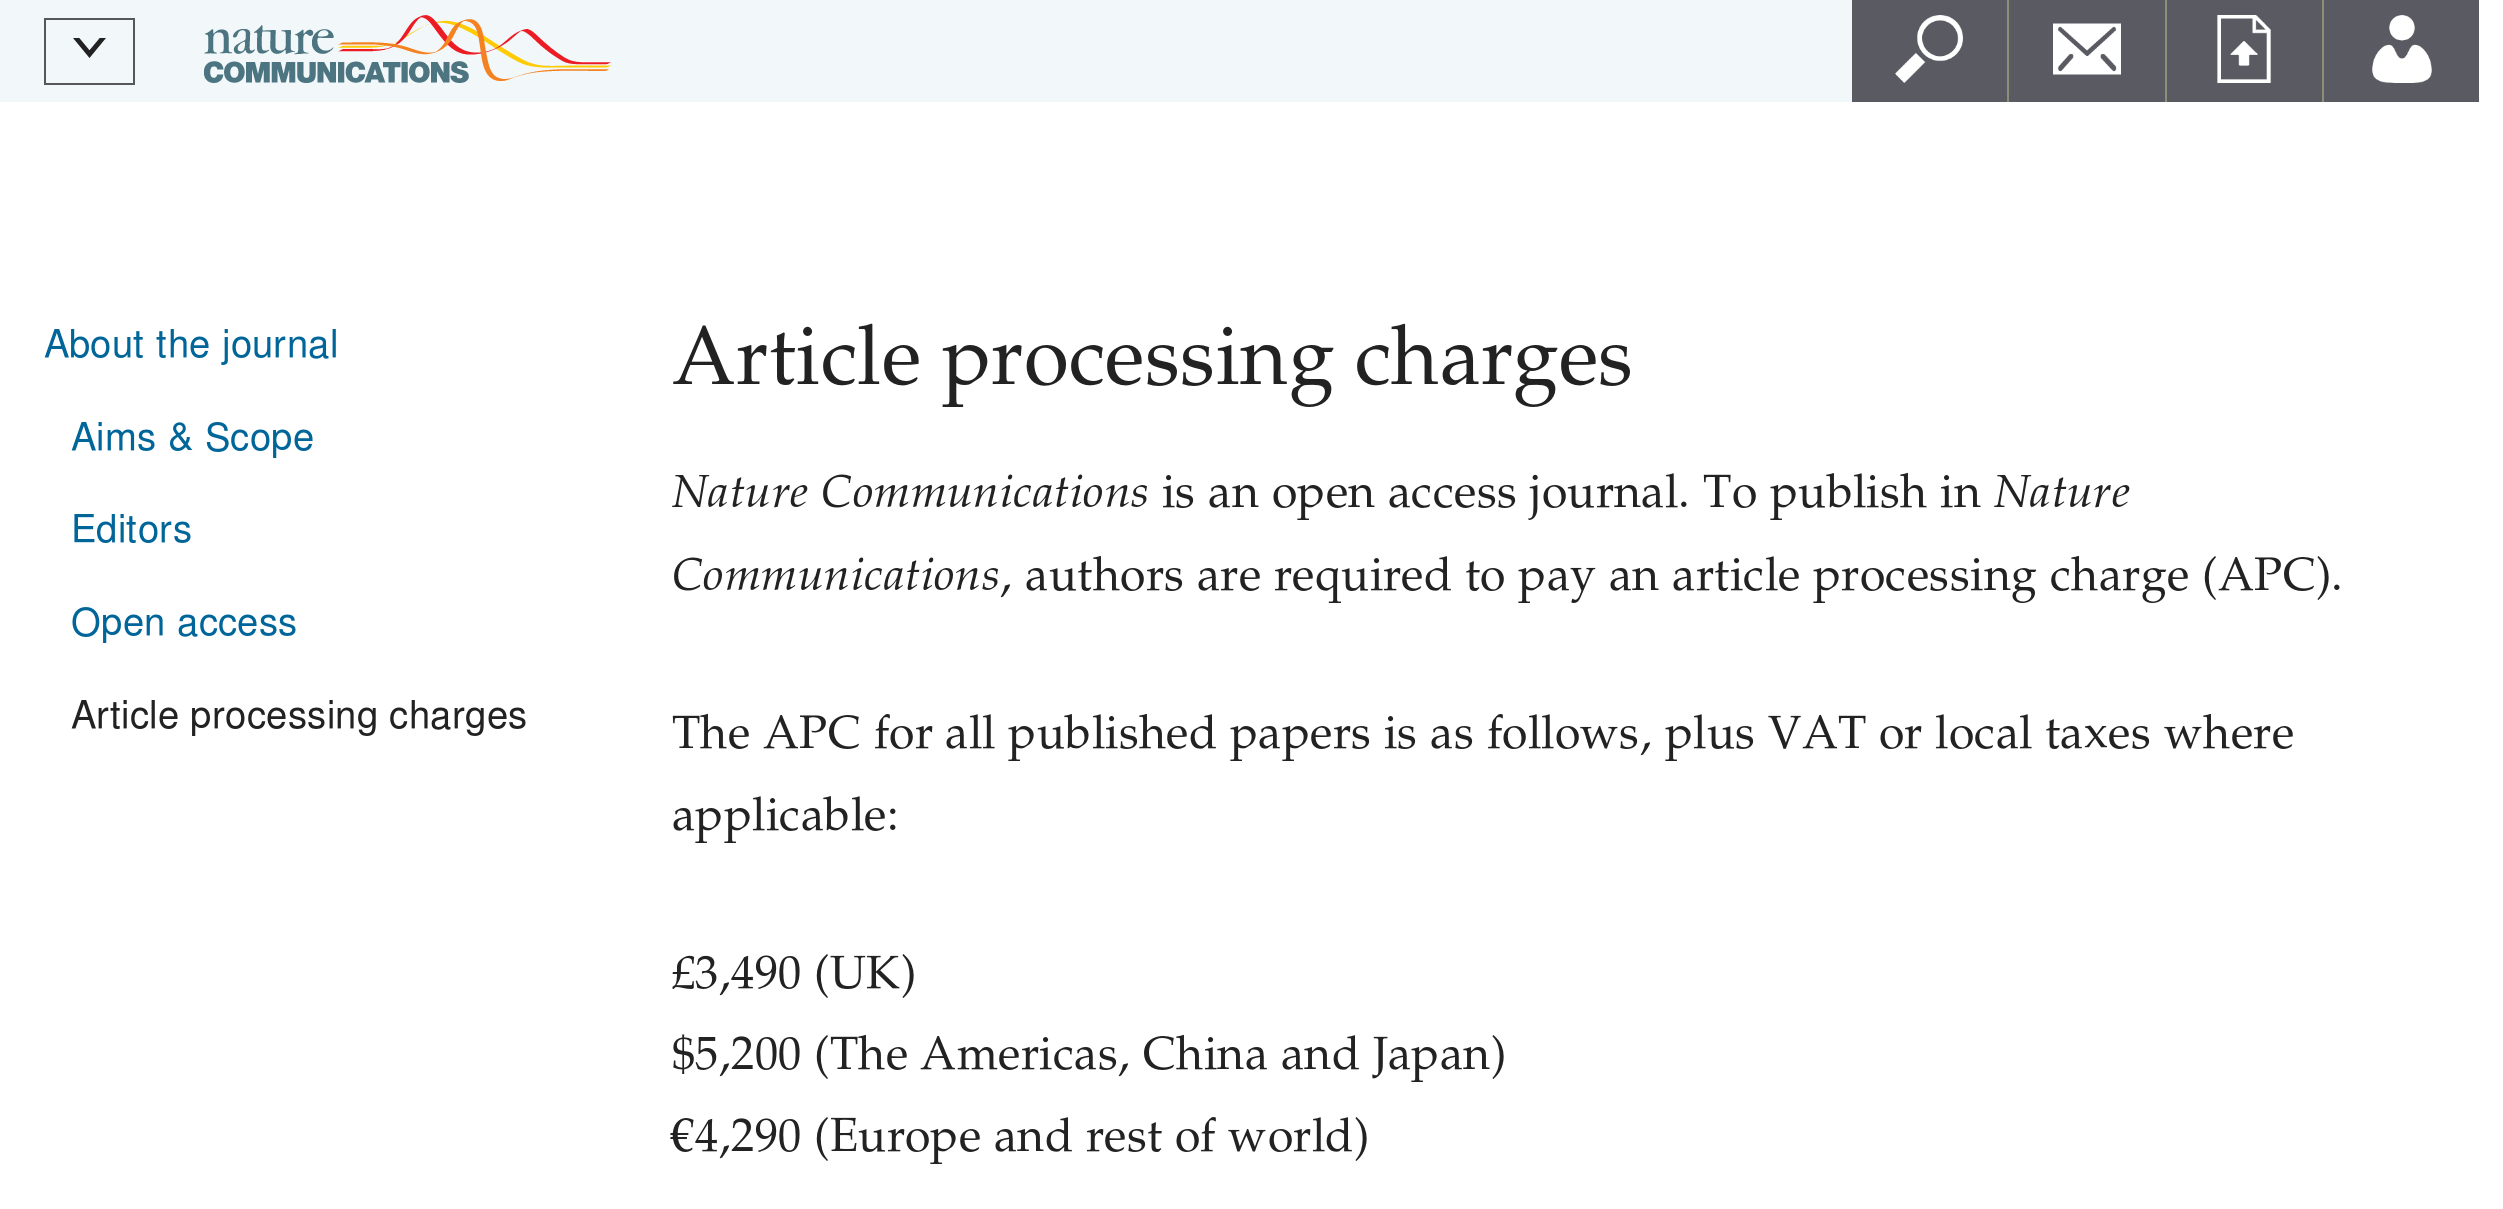
\includegraphics[width=\textwidth]{nature.png}
}

%\setcounter{framenumber}{\thelastpagemainpart}
\end{document}
